\documentclass[fleqn,usenatbib]{mnras}


\usepackage{newtxtext,newtxmath}
\usepackage{pict2e}
\usepackage[greek,english]{babel}
\usepackage[T1]{fontenc}
\usepackage{tikz}
\usepackage{pgfplots}
\usetikzlibrary{decorations.pathreplacing,calligraphy,patterns}
\usepackage{../../Papers/JML}



\title[Deforesting]{Deforesting Coverage Data}
\author[J. Fraser-Govil]{Jack Fraser-Govil
}

\def\commentVisible{1}

\begin{document}

	\label{firstpage}
	\pagerange{\pageref{firstpage}--\pageref{lastpage}}
	\maketitle
	
	\section{Introduction \& Motivation}
	
		Coverage data belies a wealth of data -- we have already seen that a hidden set of biases can be seen when considering the coverage-frequency distribution. 

		In addition, Coverage can also be used to detect the presence of large-scale copy-number variations and other forms of duplication or deletion (which we shall generically call `gains' and `losses'). In the case of losses it is easy to see why this would be the case, it is perhaps less obvious why it happens in the case of gains.
		
		Provided the read length is smaller than the scale of the duplications we are interested in, it is generally not possible to infer which copy of a motif a read originated from, and so the alignment does not record this as an insertion/duplication of bases -- it simply assigns them to the original copy in the reference, leading to a spurious over-coverage of the reference, as shown in Figure \ref{Fig:Diagram}.

		Only reads which bridge the gap between consecutive copies would permit us to properly infer the presence of duplication -- however, if the number of duplicates is greater than two, then there are multiple such bridge points, and the problem is highly degenerate and we must rely on the coverage to infer the number of duplications. 
		
		The problem with this kind of inference is that Coverage is already inherently stochastic and highly noisy - coverage plots covering any significant portion of the genome are difficult to interpret due to a large degree of shot noise which -- as we have seen -- has a significantly higher dispersion than Poisson shot noise, with the noise changing on (approximately) a per-base resolution. 

		Plots of the base coverage are - to be charitable - hard to interpret, reminiscent of the notorious `Lyman-Alpha forest' in astrophysical spectroscopy. Whilst large-scale trends can (just about) be picked out by eye, we might desire a more rigorous and sophisticated methodology.  

		The aim of this work is to generate a computational tool which can peer through the `Forest', and see the underlying pattern.
		\begin{figure}
			\begin{center}
				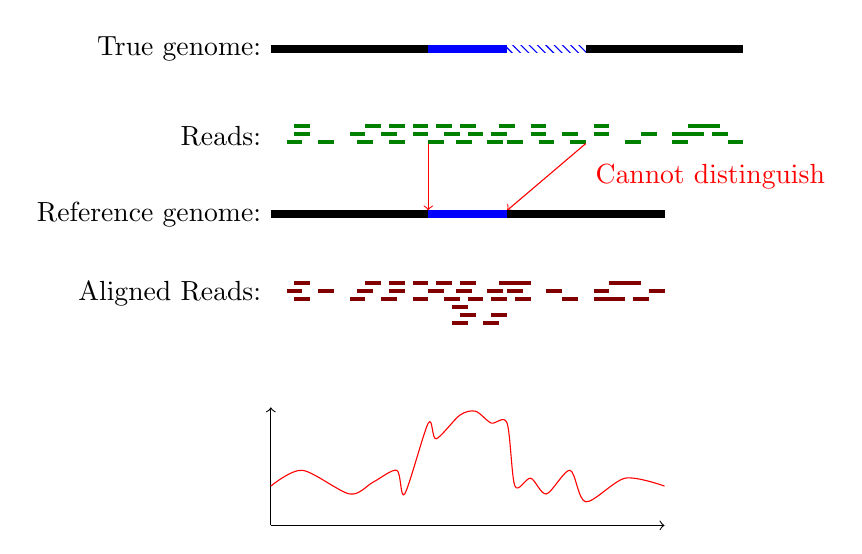
\begin{tikzpicture}
					\node[anchor=east] at (0,0.05) {True genome:};
					\fill (0,0) rectangle (2,0.1);
					\fill[blue] (2,0) rectangle (3,0.1);
					\fill[blue,pattern=north west lines, pattern color=blue] (3,0) rectangle (4,0.1);
					\fill (4,0) rectangle (6,0.1);

					\def\readheight{-1}
					\node[anchor=east] at (0,{\readheight-0.05}) {Reads:};

					\foreach[count=\i] \x in {0.3,1,1.4,1.8,2.2,2.5,2.8,3.3,3.7,4.1,4.7,5.1,5.3,5.6}
					{
						\fill[green!50!black] (\x,\readheight) rectangle ({\x+0.2},{\readheight -0.05});
					}
					\foreach[count=\i] \x in {0.2,0.6,1.1,1.5,2,2.35,2.75,3,3.4,3.8,4.5,5.1,5.8}
					{
						\fill[green!50!black] (\x,{\readheight-0.1}) rectangle ({\x+0.2},{\readheight -0.15});
					}
					\foreach[count=\i] \x in {0.3,1.2,1.5,1.8,2.1,2.4,2.9,3.3,4.1,5.3,5.5}
					{
						\fill[green!50!black] (\x,{\readheight+0.1}) rectangle ({\x+0.2},{\readheight +0.05});
					}
					\def\refheight{-2}
					\draw[->,red] (2,\readheight-0.15)--(2,\refheight);
					\draw[->,red] (4,\readheight-0.15)--(3,\refheight);
					\node[anchor=west,red] at (4,{(\refheight+\readheight-0.15)/2}) {Cannot distinguish};
					\node[anchor=east] at (0,{\refheight -0.05}) {Reference genome:};
					\fill (0,\refheight) rectangle (2,{\refheight -0.1});
					\fill[blue] (2,\refheight) rectangle (3,{\refheight -0.1});
					\fill (3,\refheight) rectangle (5,{\refheight -0.1});

					\def\areadheight{-3}
					\node[anchor=east] at (0,{\areadheight-0.05}) {Aligned Reads:};

					\foreach[count=\i] \x in {0.3,1,1.4,1.8,2.2,2.5,2.8,3.3,3.7,4.1,4.7,5.1,5.3,5.6}
					{
						\def\xoffset{0}
						\def\yoffset{0}
						\newdimen\pos
						\pos = \x cm
						\ifdim \pos > 3cm
							\def\xoffset{1}
							\ifdim \pos < 4cm
								\def\yoffset{0.3}
							\fi
						\fi
						\fill[red!50!black] ({\x-\xoffset},{\areadheight -\yoffset-0.1}) rectangle ({\x-\xoffset+0.2},{\areadheight -\yoffset-0.15});
					}
					\foreach[count=\i] \x in {0.2,0.6,1.1,1.5,2,2.35,2.75,3,3.4,3.8,4.5,5.1,5.8}
					{
						\def\xoffset{0}
						\def\yoffset{0}
						\newdimen\pos
						\pos = \x cm
						\ifdim \pos > 3cm
							\def\xoffset{1}
							\ifdim \pos < 4cm
								\def\yoffset{0.3}
							\fi
						\fi
						\fill[red!50!black] ({\x-\xoffset},{\areadheight -\yoffset}) rectangle ({\x-\xoffset+0.2},{\areadheight -\yoffset-0.05});
					}
					\foreach[count=\i] \x in {0.3,1.2,1.5,1.8,2.1,2.4,2.9,3.3,4.1,5.3,5.5}
					{
						\def\xoffset{0}
						\def\yoffset{0}
						\newdimen\pos
						\pos = \x cm
						\ifdim \pos > 3cm
							\def\xoffset{1}
							\ifdim \pos < 4cm
								\def\yoffset{0.3}
							\fi
						\fi
						\fill[red!50!black] ({\x-\xoffset},{\areadheight -\yoffset+0.1}) rectangle ({\x-\xoffset+0.2},{\areadheight -\yoffset+0.05});
					}


					\def\plotheight{-6}
					\draw[->](0,\plotheight)--(5,\plotheight);
					\draw[->](0,\plotheight)--++(0,1.5);
					\draw [red] plot [smooth] coordinates {(0,{\plotheight+0.5}) (0.4,{\plotheight+0.7}) (1,{\plotheight+0.4}) (1.3,{\plotheight+0.55}) (1.6,{\plotheight+0.7}) (1.7,{\plotheight+0.4})
						(2,{\plotheight+1.3})  (2.1,{\plotheight+1.1})  (2.4,{\plotheight+1.4})  (2.6,{\plotheight+1.45}) (2.8,{\plotheight+1.3})	(3,{\plotheight+1.3})  
						(3.1,{\plotheight+0.5}) (3.3,{\plotheight+0.6}) (3.5,{\plotheight+0.4}) (3.8,{\plotheight+0.7}) (4,{\plotheight+0.3}) (4.5,{\plotheight+0.6})  (5,{\plotheight+0.5})    
						};
				\end{tikzpicture}
			\end{center}\caption{A depiction of duplication leading to a higher coverage. The blue hatched region is duplicated with respect to the reference, but since the reads are much shorter than the duplicated region, they cannot be properly assigned as duplicates, instead leading to a higher coverage rate.}\label{Fig:Diagram}
		\end{figure}

	\section{Mathematical Theory}

		\subsection{Naive Smoothing}

			The most obvious solution is to simply pass a smoothing kernel over the data, and use that to infer the underlying mean function that the data is oscillating around. The Nadarya-Watson (cite?) method uses a kernel function $K_\lambda(x,y) = \frac{1}{\lambda} k\left(\frac{|x-y|}{\lambda}\right)$, and the mean estimate of a set of data $(x_i,y_i)$ is given by:
			\begin{equation}
				\hat{m}_\lambda(x) = \frac{\sum_i^n K_\lambda(x,x_i) y_i}{\sum_i K_\lambda(x,x_i) }
			\end{equation}
			The kernel should be sufficiently decaying that $K_\lambda(x,y) = 0$ when $|x-y| \gg \lambda$, where $\lambda$ is a characteristic `smoothing lengthscale'.

			Smoothing in this fashion serves as a generic way to extract a smooth curve from the extremely noisy data present (i.e. the `forest') - however it fails us on a number of grounds:
			\begin{itemize}
				\item It is not biologically motivated (no underlying mechanism present), without regard to any other information we have about the system.
				\item It reduces the coverage to a smooth curve. This is undesirable because:
				\begin{itemize}
					\item It gives us no indication about where the gains and losses begin or end (the quantity of real interest to us) -- we would need to do some more statistical post-processing in order to infer the edges of the transitions. The smoothing only helps human eyes see things, it does not particularly help in our numerical affairs.
					\item The action of the kernel is (by definition) to smooth out sharp transitions. However -- when a transition occurs we \textit{expect} it to be a sharp transition. The kernel method necessarily smooths out these edges -- it is difficult to distinguish between `noise' and `genuine transitions'.
				\end{itemize}
			\end{itemize}

		% \subsection{Poisson Fitting}

		% 	A more scientific (and less `let's just draw a line through the data') method would exploit the fact that we know the data should (more or less) follow a Poisson distribution. The advantage (other than just aesthetic) of this over the mean-smoothing approach is that the Poisson distribution (and indeed, any realistic coverage distribution) is asymmetric around the peak value -- the Poisson covers the semi-infinite interval $[0,\infty]$. Therefore, although we should expect the sample mean of a Poisson to be equal to the Poisson Parameter $\lambda$, deviations away from this are asymmetric in a way that the Kernel smoothing mechanism might have trouble with.
			
		% 	From previous work we know that the distribution is non-Poissonic on a global scale (i.e. the entire chromosome/genome). However, we might hypothesise that the distribution is obeyed \textit{locally}, but with variations in the mean of the distribution over the spatial extent of the chromosome. In this case, the probability distribution of the coverage at index $i$ is:
		% 	\begin{equation}
		% 		p(k,i) = \frac{\left[\lambda(i)\right]^k e^{-\lambda(i)}}{k!}
		% 	\end{equation}
		% 	The deforestation exercise therefore reduces to inferring the behaviour of $\lambda$, given the observed distribution.

		% 	We assume that we have some way of parameterising the function $\lambda(i) = \lambda(i,\vec{\theta})$, and so we wish to infer the parameters $\theta$ which maximise the following Likelihood:
		% 	\begin{spalign}
		% 		\mathcal{L}(\vec{\theta},\{i,y_i\}) & = \sum_i \left[ y_i \ln(\lambda(i|\vec{\theta})) - \lambda(i|\vec{\theta}) - \ln(y_i!) \right] + \text{Prior}(\vec{\theta})
		% 		\\
		% 		& = \text{const} + \sum_i \left[ y_i \ln(\lambda(i|\vec{\theta})) - \lambda(i|\vec{\theta})\right] + \text{Prior}(\vec{\theta})
		% 	\end{spalign}
		% 	This has gradient:
		% 	\begin{equation}
		% 		\pdiv{\mathcal{L}}{\vec{\theta}} = \sum_i \left( \frac{y_i}{\lambda(i|\vec{\theta})} - 1\right) \pdiv{\lambda(i|\vec{\theta})}{\vec{\theta}}
		% 	\end{equation}
		% 	Hence a basic gradient descent method can easily find the most likely distribution -- modulo some prior which enforces smoothness. 

		% 	This, however, has a similar problem to the Naive fitting method: when the Prior is weak, it is just as noisy as the data. When the prior is strong, it simply smooths over all but the largest deviations, and does not have sharp transition edges which would allow us to identify the position of gains and losses.

		% 	\subsubsection{A Note On Priors}
				
		% 		The most obvious Prior for imposing the kind of smoothness we are looking for is something on the form:
		% 		\begin{equation}
		% 			\log\text{Prior}(\lambda(\theta)) = - \sum_i \frac{(\lambda_i - \lambda_{i-1})^2}{\ell^2}
		% 		\end{equation}

		% 		This works, insofar as it imposes a penalty whenever subsequent values of $\lambda$ are far apart from each other, and smaller when they are close together -- but has the problem of `fine tuning': the prior has a `strength' as an external parameter, which then controls the `spikiness' of the output curve. By selecting this value appropriately, the user is able to either make the output ust as much of a forest as the input data, or perfectly smooth: and anything in between. 

		% 		The user is then left to fine tune the dials of this parameter until they get something they would find acceptable. The problem with this is that it invariably leaves the user projecting their own expectations on the input -- you only get out what you put in. 

		% 		In such a case, a Bayesian statistician would say that we have formulated our Prior poorly -- it has a free parameter (the strength), over which we have actually no prior knowledge. In fact, on further examination the strength (formulated as a length scale over which the binding happens) isn't even the quantity we are wishing to constrain since -- as we have already noted -- we don't even want a smooth output curve.
			
			
		% 		We must therefore ask what it is we wish our smoothing-prior to do since it evidently isn't `smoothing' -- since we are looking for a highly discontinuous output function! We want our prior to be such that it causes the model to disregard small-scale oscillations in the coverage as merely being noise. Smoothing length scales had this as a side effect -- but with the unfortunate side effect that they also smoothed over what we (probably) believe to be sharp, discontinuous edges. 

		% \subsection{Attempt 3: Harmonic Fitting}

		% 	The problem with the prior attempts is that they attempt to fit some continuous function to the data, in the hope of elucidating some distinct upward and downward steps in the data, which represent `gains' and `losses' -- in so doing they are messy and noisy, and only marginally easier to interpret than the raw data. 

		% 	We should like a method which actually assigns discrete values, and hence makes it easier to mechanistically identify regions of gains and losses in the genome. We should also like the Priors which we place on the models to be relevant to the quantities which we are actually studying: rather than attempting to smooth out noise via some arcane length scale, we should instead place strict boundaries on what we do and do not consider relevant.

		% 	We propose the following solution, which takes inspiration from the `harmonics' observed in musical instruments: when you play an `A' on a piano, you do not merely produce a pure tone at 440Hz, but a superposition of \textit{harmonics} of that tone: at 880Hz, 1320HZ and so on. 

		% 	So it is with our hypothesis: we are asserting that there is a single, mean coverage depth but that, due to the effects of normal heterogeneity and subsequent gains and losses, parts of the genome are being amplified or suppressed. This results in `harmonics' of the mean coverage depth: integer multiples of the `fundamental harmonic'

		% 	Hence, we should only fit a single frequency, but with the knowledge that each datapoint should then be fit to a integer harmonic of that frequency.

		% 	The model probability of a datapoint occuring due to the $q^\text{th}$ harmonic of some fundamental frequency $\nu$ is:
		% 	\begin{spalign}
		% 		p(k|\nu) = \left(\frac{\left[q\nu\right]^k e^{-q\nu}}{k!}\right)
		% 	\end{spalign}
		% 	Therefore the likelihood of a given harmonic $q \in \mathbb{N}$ ($q$ must be a non-negative integer to satisfy the harmonic constraint) is:
		% 	\begin{spalign}
		% 		\mathcal{H}(q) &= p(q|k,\nu) 
		% 		\\
		% 		& = \frac{p(k|q,\nu) p(q)}{p(k)}
		% 		\\
		% 		& = \frac{\left[q\nu\right]^k e^{-q\nu}}{k!} \times \text{Prior}(q)
		% 	\end{spalign}
		% 	The most likely value of $q$ can therefore be found by a simple integer search: this is technically an infinite task, but we can restrict ourselves to a finite subset via our prior.		This is a statement of Bayesian maximum Likelihood: we search for the most likely value of $q$, which is determined both by the data and our knowledge of what a reasonable value of $q$ is. The restriction of $q$ to the natural numbers (which we define to include 0) is the `harmonic' assumption: everything should exist in multiples of the fundamental frequency.

		% 	We expect that most sequences in the DNA will have $q = 2$, i.e. they occur only once on each copy of the chromosome. A deletion (or a heterozygous sequence) on one chromosome will give $q = 1$, and a deletion on both chromosomes give $q = 0$. An amplification likewise gives $q = 3$ if the sequence is duplicated on one only chromosome and so on.
			
		% 	It is worth noting that we are detecting the absolute multiplicity, rather than the relative: Motifs which have multiplicity in the reference (such as in the centromere or telomere) will show up as high-$q$ values, and low $q$ values will appear where mis-alignment has occurred. Therefore motifs which are already repetitive but which have suffered gains or losses will move from one $q$ to another -- we will only be able to detect these regions by comparing to a healthy sample. 


		% 	\subsubsection{Improving the model}

		% 		We have formulated a basic probability assignment model using harmonics but if we were to apply this directly to the data we would find a number of problems since, at the moment, it applies only on a resolution of an individual base. A base with a coverage of 2 might be assigned a $q = 0$ (or not, as we shall see), whilst every other adjacent base has a $q = 10$ -- we need to be able to account for noise. 

		% 		The simplest way to do this is to discretise the data and find the most likely value of $q$ for a block of bases of some length $L$, assign that a $q$ and then move onto the next block. This has the problem that any transitions which occur in the middle of the block might get missed, and so the `position' of the transition is dependent on the resolution of the model which is less than desirable. 

		% 		We shall find a way around this by a proper formulation of our Prior.

		
		% 		We also note that in a region where a deletion has genuinely occurred there might still be `peaks' in the coverage due to spurious alignment or contamination from a small population of cells without the total deletion which ruins our `pure harmonic' assumption. This is a problem since even in the case of a `block' of datapoints over a total deletion is total, the probability model will never be able to pull down a region containing non-zero data to a value of $q=0$: a prior cannot force something impossible to become possible!

		% 		We must therefore refine our probability model slightly. 

		% 	\subsubsection{Error-Prone Probability Model}

		% 		There are two possible sources of additional noise which we handle slightly differently. The first source of noise is an inherent deviation from the underlying Poisson assumption - this follows from our previous work that the distribution is highly non-Poisson for a variety of reasons: we term this \textit{process noise}, and it is a fundamental part of the underlying biology. The second source is \textit{experimental noise} - contamination from different cell populations, misalignments and so on.

		% 		The process noise we model by assuming that the underlying Probability model is, instead of being a pure-Poisson, marginalised against a Gamma distribution with mean $\mu$ and variance $\sigma^2$ (in the common parameterisation this is $(\alpha,\beta) = \left(\frac{\mu^2}{\sigma^2}, \frac{\mu}{\beta^2}\right)$):
		% 		\begin{spalign}
		% 			p(k|\mu,\sigma) & = \int_0^\infty p(k|\lambda) p(\lambda|\mu,\sigma) \d \lambda 
		% 			\\
		% 			& = {NB}\left(k; \frac{\mu^2}{\sigma^2}, \frac{\mu}{\mu + \sigma^2} \right)
		% 			\\
		% 			& \left( NB(k,r,p) = \frac{\Gamma(k+r)}{k! \Gamma(r)} (1-p)^k p^r \right)
		% 		\end{spalign}
		% 		Where $NB(k;n,r)$ is the usual Negative Binomial distribution, written in terms of Real (rather than integer) $r$, and $\Gamma(x)$ is the usual Gamma function. This resulting distribution has mean $\mu = q\nu$ (recall: this was the mean value of the coverage depth) but variance $\mu + \sigma^2$ - and so we see that our distribution is Poisson-esque, albeit with a higher variance.

		% 		The Harmonic assumption is therefore embedded in this internal function: $\mu_i = q \nu$, where $q$ is an integer. We assume that $\sigma^2$ is a global constant.

		% 		However, although this has the effect of broadening the tails of the distribution (and hence making the inference much more accepting of deviations away from the expected mean), it does not help the $q=0$ problem, since $NB(k,0,p) > 0$ only if $k = 0$. In order for that, we must sum over the probability that $k$ was assigned erroneously:
				
		% 		The probability that $p(k_\text{obs}|q)$ is therefore found from:

		% 		\begin{equation}
		% 			p(k_\text{obs}|k,\nu,\sigma^2) =\left( \sum_{k} {NB}\left(k; \frac{q^2\nu^2}{\sigma^2}, \frac{q\nu}{q\nu + \sigma^2} \right) \times p(k_\text{obs}|k)\right)
		% 		\end{equation}

		% 		For simplicity's sake, it is probably easiest to use the $L_1$ kernel:
		% 		\begin{equation}
		% 			p(k_\text{obs}|k) = \mathcal{N}\exp(-\gamma |k_\text{obs} - k|)
		% 		\end{equation}

		% 	\subsubsection{The Prior}

		% 		In order to properly formulate a Prior, we must first give some thought about exactly what question we are trying to answer. We are trying to ascertain the `harmonic' at each index of the genome, given the observed coverage -- but we want the model to disregard small-scale oscillations in the coverage as merely being noise. Smoothing length scales had this as a side effect -- but with the unfortunate side effect that they also smoothed over what we (probably) believe to be sharp, discontinuous edges. 

		% 		Let us therefore use this as a strict prior: there should be no oscillations on a scale shorter than some enforced length scale $L$ - we assert that any gains or losses which span $L$ bases or fewer are merely noise. Any determination if a change in harmonic has occurred must therefore consider \textit{at least} $L$ bases. 

		% 		A standard Bayesian hypothesis can be formulated at the index $i$ to determine if there has been a transition by considering the Hypothesis ``the harmonic on the domain $[q,q+L]$ is equal to $q_i$'', and testing all reasonable values of $q_i$ (we suggest between 0 and 10 as being reasonable values). The odds-Likelihood of a transition is then:
		% 		\begin{equation}
		% 			p(\text{transition } q_{i-1} \to q) = \frac{p(D_i\to D_{i+L| q})}{p(D_i\to D_{i+L| q_{i-1}})} \times \text{Prior}(q | q_{i-1})
		% 		\end{equation}
		% 		It simply suffices to find if any of these terms is greater than 1 and, if any, which is the largest: this is the assigned value of $q$. The prior then allows us to penalise `marginal' jumps by only assigned jumps when the evidence reaches a threshold:
		% 		\begin{equation}
		% 			\text{Prior}(q | q_{i-1}) = \begin{cases} 0 < \alpha \leq 1 & \text{ if } q = q_{i-1}
		% 			\\
		% 		1 & \text{else}\end{cases}
		% 		\end{equation}
		% 		The case where $\alpha \approx 1$ means we accept a transition when the evidence is very marginal, $\alpha \ll 1$ means we require an overwhelming amount of evidence. Given some of the other post-processing that we will be doing (to locate transition edges more precisely), and provided $L$ is sufficiently large that most spurious jumps will be eliminated, we use $\alpha = 0.5$ as a good first port of call.

		% 		Should we find that $q \neq q_{i-1}$, we have therefore been able to robustly identify that there is a transition in the region $[i,i+L]$ - but it is not true that the transition edge is at $i$ -- if $\alpha = 1$ the transition is probably somewhere in the middle of the region, whilst as $\alpha \to 0$ it gets closer to $i$. To robustly identify the edge of the transition we need to do a second hypothesis test -- that the transition $q_{i-1} \to q$ occurs at an index $j$, the Likelihood of which is computed as:
		% 		\begin{equation}
		% 			\mathfrak{p}(\text{transition at} j | i, \text{data, }D) = p(D_i \to D_{j-1} | q_{-1} ) \times p(D_j \to D_{j + L} | q)
		% 		\end{equation}
		% 		I.e., we sucessively compute the probability that every point left of $j$ is at the original $q=q_{i-1}$, and every point to the right is at the new value of $q$: the one with the highest value of $\mathfrak{p}$ is where we assign $j$.


		% 	\subsubsection{Initial Frequency Detection}

		% 		The most important free variable in our model is $\nu$, the fundamental frequency of the model. 

		% 		If we erroneously assign $\nu$, the model produce results which veer towards the nonsensical since the majority of the data will lie off-harmonic, and so the model will place transitions at more or less spurious points. We can mitigate some of this problem by a gradient descent approach -- however we note that due to the discontinuous nature of the assignments that this is only useful if our initial guess is good. 

		% 		We can also trivially see that there is a high degree of degeneracy in the assignment of $\nu$ since $\nu \to \nu/10$, $q \to 10q$ produces identical results -- albeit at the cost of reducing the power of our Harmonic approach, since it relies on the fact that the harmonics are highly distinct -- our prior in this case is that the majority of the genome should have $q=2$, being a normal non-heterogenous DNA sequence.


		% 		We propose that the following algorithm would identify the best possible starting value for $\nu$:
		% 		\begin{itemize}
		% 			\item Start with $\nu = 1$ (or other small value)
		% 			\item Assign $q$s across the dataset without using 
		% 		\end{itemize}


		\subsection{Harmonic Fitting}

			The primary problem with the na\"ive smoothing approach was that it (by definition) \textit{smoothed out} the data, in order that we might more easily spot \textit{discontinuities} in the data. These two points -- smoothing and discontinuities -- stand in direct opposition to each other, and so the method is inherently flawed.

			We should therefore attempt to identify the discontinuities straight from the dataset. This, in essence is a form of \textit{step detection}, a well known problem in signal processing. However, whilst there exist several out-of-the-box algorithms which might provide us with robust detections, we note that knowledge about the form of the data can be leveraged to provide a significantly more powerful and biologically meaningful inference. 
			
			\subsubsection{Model Assumptions}
			
				We use the following knowledge and assertions as the underpinnings of our model:

				\begin{enumerate}
					\item The distribution of coverage, $k$, is approximately Poisson-like, around some central value $\lambda$
					\item The value of $\lambda$ is constant across a chromosome, except during gains or losses, where it changes discontinuously
					\item The gains and losses occur throughout the sample (i.e. no subclonality)
					\begin{itemize}
						\item As a result, duplication or deletion of a region results in $\lambda$ changing by integer multiples (`harmonics', denoted as $q$) of an underlying `fundamental frequency', $\nu$.
						\item Most of the sample should have a harmonic of $q = 2$ - normal human diploidy.
					\end{itemize}
					\item Discontinuities must be separated by at least a distance $L$ on the linear genome, else they would have been resolved by the alignment.
					\item There is some error in the alignment method\footnote{This is most important in regions of deletion, since $\lambda = 0$ is very difficult to infer if even a single read is misaligned into a deleted region}, such that a base assigned coverage $k_\text{obs}$ actually had coverage $k_\text{true}$.
					\item We should prefer a model with fewer jumps to one with more, all else being equal.
				\end{enumerate}
			
				The key assumption here is iii: the assumption that changes in coverage occur in \textbf{integer steps} of the fundamental frequency $\nu$, such that the average coverage in a region is always $q \nu$, where $q$ is our integer `harmonic'. It is this distinction which makes our step-detection algorithm highly distinct from other methods. 

				It is worth noting that we are only able to detect the \textit{absolute} harmonic, rather than the relative: Motifs which have multiplicity in the reference (such as in the centromere or telomere) will show up as high-$q$ values, and low $q$ values will appear where mis-alignment has occurred. Therefore motifs which are already repetitive but which have suffered gains or losses will move from one $q$ to another -- we will only be able to detect these regions by comparing to a healthy sample. 
				
				The task of detecting the `steps', therefore, requires that we assign each base a value of $q$: gains and losses are trivially detectable wherever this integer value changes.

			\subsubsection{Statistical Model}

				In order to assign the values of $\{q\}$ to a set of genome coverage data $\{k\}$, we must find a way of assigning a statistical score, $\mathcal{L}$ to a proposed set of harmonics, $\{q\}$. The task of step-detection then reduces to finding the value of $\{q\}$ which maximises $\mathcal{L}$, and is therefore the most likely given the observed data.

				We make the standard assumption that the coverage $k_i$ of the $i^\text{th}$ base is drawn independently and identically from an underlying distribution function (\textit{iid}), which is a function of the fundamental frequency, $\nu$, and the harmonic, $q_i$. Bases are statistically connected through the \textit{prior} function, which encodes many of the points outlined in the previous section. 
				
				As a result of the \textit{iid} assumption, the global score can be found to be:

				\begin{equation}
					\mathcal{L}(\{q\} | \{k\}, \nu) = \sum_i \mathfrak{p}\left(k_i | q_i, \nu \right) + \text{Prior}(\{q\}) \label{E:Score}
				\end{equation}

				This is an indirect statement of standard Bayesian Maximum Posterior methodology - the quantity $\mathfrak{p}$ is the log-probability of observing the data $k_i$ given the harmonic $q_i$ and parameter $\nu$. 

				The probability $p(k_i | q_i,nu)$ can be formulated from our assumptions - namely that we are looking for an `error prone', Poisson-like distribution. There are two possible sources of additional noise which we handle slightly differently. The first source of noise is an inherent deviation from the underlying Poisson assumption - this follows from our previous work that the distribution is highly non-Poisson for a variety of reasons: we term this \textit{process noise}, and it is a fundamental part of the underlying biology. The second source is \textit{experimental noise} - contamination from different cell populations, misalignments and so on.

				The process noise we model by assuming that the underlying Probability model is, instead of being a pure-Poisson, marginalised against a Gamma distribution with mean $\mu$ and variance $\sigma^2$ (in the common parameterisation this is $(\alpha,\beta) = \left(\frac{\mu^2}{\sigma^2}, \frac{\mu}{\sigma^2}\right)$):
				\begin{spalign}
					p(k|\mu,\sigma) & = \int_0^\infty p(k|\lambda) p(\lambda|\mu,\sigma) \d \lambda 
					\\
					& = {NB}\left(k; \frac{\mu^2}{\sigma^2}, \frac{\mu}{\mu + \sigma^2} \right)
					\\
					& \left( NB(k,r,p) = \frac{\Gamma(k+r)}{k! \Gamma(r)} (1-p)^k p^r \right)
				\end{spalign}
				Where $NB(k;n,r)$ is the usual Negative Binomial distribution, written in terms of Real (rather than integer) $r$, and $\Gamma(x)$ is the usual Gamma function. 
				
				The \textit{experimental noise} we model in a more simplistic fashion, since it is possible for artefacts such as misalignment to cause wild deviations in the coverage distribution - we therefore assign a uniform noise between $k=0$ and some sufficiently large $K$, with weight $\gamma$. As a result, the full probability distribution is:

				\begin{equation}
					p(k|\mu,\sigma,\gamma,K) = (1- \gamma)  {NB}\left(k; \frac{\mu^2}{\sigma^2}, \frac{\mu}{\mu + \sigma^2} \right) + \begin{cases} \frac{\gamma}{K} & k < K \\ 0 &\text{else}\end{cases}\label{E:Probability}
				\end{equation}
				
				This resulting distribution has mean $\langle k \rangle = (1-\gamma)\mu + \frac{\gamma K}{2}$ -- so long as $\mu \gg \gamma K$, this therefore will closely resemble the sample mean. However, when $\mu = 0$ it has the desirable property of allowing a non-zero sample mean.

				The Harmonic assumption is embedded in the assumption tha we will always use $\mu_i = q \nu$, where $q$ is an integer. We assume that $\sigma^2$, $K$ and $\gamma$ are a global constants.

				Figure \ref{Fig:Distributions} shows some examples of this distribution (the `Errored-Binomial') compared to the basic Poisson Distribution and the Negative Binomial distribution, demonstrating its desirable properties.

				\begin{figure}
							\includegraphics*[width=\linewidth,keepaspectratio=true]{Distribution.png}
							\caption{Various distribution functions: Poisson, Negative Binomial (NB) and our `Errored-Binomial' (EB) are shown with various parameters, and $\mu =30$ (top panel) and $\mu = 0$ (lower panel). The key feature of the EB distribution is that it resembles the NB distribution near the peak, but has wider wings -- most notably when $\mu = 0$ (corresponding to total deletion), where the Poisson and NB distributions are zero everywhere except $k=0$, whilst the EB distribution permits non-zero values. As a result, the EB-distribution has a mean slightly greater than zero -- $\mu$ refers to the `true sampling' mean, rather than the observed.}\label{Fig:Distributions}
						\end{figure}
			
				Finally, we must formulate a suitable prior, which enforces the remainder of our assumptions, namely:
				\begin{enumerate}
					\item Consecutive values of $q_i$ should be similar
					\item Changes in $q_i$ can only happen over a large distance
					\item Most of the genome should be at $q_i = 2$ (equal to the ploidy)
				\end{enumerate}
				Therefore, we propose:
				\begin{spalign}
					\text{Prior}(\{q\})   = & \sum_i \Bigg[  \mathfrak{p}_\text{ploidy} u(q_i,2)  
					\\
					 + & u(q_i,q_{i-1})\left( \mathfrak{p}_\text{jump} +  \mathfrak{p}_\infty \sum_{j = i-L}^{i-1} u(q_j,q_{i-1})  \right)\Bigg]
					 \\
					 u(a,b) = \begin{cases}
						0 & \text{a = b}
						\\
						1 & \text{else}
					 \end{cases}\label{E:Prior}
				\end{spalign}
				The terms in the prior therefore act (in order), to penalise every base which is not at the expected diploid level by an amount $\mathfrak{p}_\text{diploid}$, penalise every jump between dissimilar $q$s by an amount $\mathfrak{p}_\text{jump}$ and to penalise jumps which occur within a distance $L$ of another jump by an amount $\mathfrak{p}_\infty$, which is a number\footnote{A surreal number, in fact} $\approx -\infty$, but which has the property $0 \times \mathfrak{p}_\infty = 0$ -- rather than a penalty, this therefore acts as a \textit{forbiddance}, discarding models with such jumps.


			\subsubsection{Algorithmic Concerns}

				Equations \eqref{E:Probability} and \eqref{E:Prior} provide everything we need to compute the score \eref{E:Score} for a proposed set of $\{q\}$. We therefore now need an algorithm which provides the minimal set.

				% The Harmonic fitting method shows a vast improvement over the previous iteration - however it still suffers from a number of drawbacks, mostly associated with the somewhat dubious means by which the Bayesian tests were `bootstrapped' from each other (technically each successive probability should be fully conditioned on the previous set, rather than just stuffing that all into a simplistic prior).

				% The Harmonic Network method is an attempt to a) make the assignment robust and mathematically sound and b) devise a method which is conceptually easier to understand and follow. 

				Provided that we are able to make the assumption that there is some finite $Q$ such that $0 \leq q < Q$ across the entire genome, it is most convenient to think of the assignment of the harmonics to the genome as a \textit{network}, such that finding the optimal assignment is equivalent to finding the shortest path through the network.

				The network is arranged in a series of layers (not dissimilar in structure to the network diagrams of feedforward neural networks, whence this idea was derived) - each layer corresponding to a given base in the genome and its associated coverage value. The vertices (or `nodes', to continue the FNN analogy) in the layer then correspond to different values of $q$ that might be assigned to that base. In short, a node $n_{iq}$ corresponds to the $i^\text{\th}$ base being assigned a harmonic of $q$.

				The edges between vertices are directional (so ``$a$ is connected to $b$'' means that $a\to b$ is possible, but not $b\to a$), and obey the following rules:
				\begin{enumerate}
					\item The start node is connected to all nodes in the first layer, $n_{0q}~~ 0 \leq q < Q$ 
					\item The node $n_{iq}$ is connected to $n_{i+1,q}$ (`step edges') and $n_{i+L,j}$ (`jump edges') where $j\neq q$ (provided that $i + L < G$, the genome size)
					\item The nodes $n_{G-1,q}$ are connected to the End node
				\end{enumerate}

				Figure \ref{F:Network} demonstrates this network setup graphically. Each step edge (including those from the start node) has a cost:
				\begin{equation}
					\text{Cost}(n_{iq} \to n_{i+1,q}) = p_{\vec{\theta}}(k_i | q) + \mathfrak{p}_\text{ploidy} u(q,2)
				\end{equation}
				`Jumping' from $n_{iq} \to n_{i+L,j\neq q}$ enforces the requirement that any jumps must be larger than $L$ - traversing along a jump edge corresponds to assigning all nodes $i+1 \to i+L$ to the harmonic $j\neq q$, and hence has an associated cost:
				\begin{equation}
					\text{Cost}(n_{iq} \to n_{i+L,j\neq q}) = \mathfrak{p}_\text{jump} + \sum_{a = i+1}^{i+L} \left( p_{\vec{\theta}}(k_i | q)+ \mathfrak{p}_\text{ploidy} u(q,2) \right)
				\end{equation}
				Here we have used the shorthand $p_{\vec{\theta}}(k|q) = p(k| q\nu, \sigma,\gamma,K)$, our underlying `Errored Binomial' distribution function.

				From these rules it is a simple matter of using a basic shortest-path algorithm: step through each layer and compute the shortest path to each node in that layer, and then iterate until the end node is reached -- the shortest path through this network corresponds to a unique $\{q\}$, which is then necessarily the one which minimises $\mathcal{L}$. An example of such a minimal path is shown in Fig. \ref{F:Path}.

				\begin{figure}
					\begin{center}
						\resizebox{\linewidth}{!}{ 
						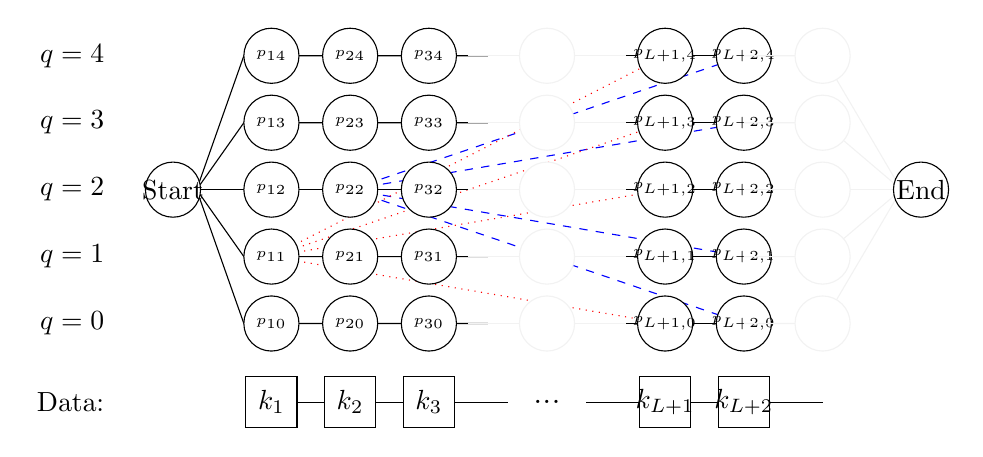
\begin{tikzpicture}
							
							\node[anchor=east] at (-2,0) {Data:};
							\draw (0,0)--++(3,0);
							\node at (3.5,0) {\large ...};
							\draw (4,0)--++(3,0);
							\def\w{0.65}
							\foreach \i in {1,...,3}
							{
								% \draw[fill=white] (\i-1,0) circle (0.35);
								\draw[fill=white] ({\i-1-\w/2},{\w/2})--({\i-1+\w/2},{\w/2})--({\i-1+\w/2},{-\w/2})--({\i-1-\w/2},{-\w/2})--cycle;
								\node at (\i-1,0) {$k_\i$};
							}
							
							
							\foreach \i in {1,...,2}
							{
								\draw[fill=white] ({\i+4-\w/2},{\w/2})--({\i+4+\w/2},{\w/2})--({\i+4+\w/2},{-\w/2})--({\i+4-\w/2},{-\w/2})--cycle;
								\node at ({4+\i},0) {$k_{L+\i}$};
							}
							
							\def\fac{0.85}
							
							\foreach \q in {0,...,4}
							{
								\def\y{\fac*\q+1}
								\if\q2
								\else
									\draw[dashed,blue] (1,{2*\fac+1})--(6,\y);
								\fi
								\if\q1
								\else
								\draw[dotted,red] (0,{1*\fac+1})--(5,\y);
								\fi
								% \if\q4
								% \else
								% \draw[dashdotted,green] (0,{4*\fac+1})--(5,\y);
								% \fi

							}
							\foreach \q in {0,...,4}
							{
								\def\y{\fac*\q+1}
								\draw (-0.95,{2*\fac+1})--(-0.35,\y)--(2.75,\y);
								\draw (4.25,\y)--(6,\y);
								\node[anchor=east] at (-2,\y) {$q=\q$};
								\foreach \i in {1,...,4}
								{
									\if\i4
										\def\c{gray!10!white}
										\draw[\c] (\i-1.5,\y)--++(2,0);
										\draw[\c,fill=white] (\i-0.5,\y) circle (0.35);
									\else
										\draw[fill=white] (\i-1,\y) circle (0.35);
										% \draw[fill=white] ({\i-1-\w/2},{\w/2})--({\i-1+\w/2},{\w/2})--({\i-1+\w/2},{-\w/2})--({\i-1-\w/2},{-\w/2})--cycle;
										\node at (\i-1,\y) {\tiny $p_{\i\q}$};
									\fi
									
								}
								\foreach \i in {1,...,3}
								{
									\if\i3
										\def\c{gray!10!white}
										\draw[\c] (\i+3,\y)--++(1,0)--(8,{2*\fac+1});
										\draw[\c,fill=white] (\i+4,\y) circle (0.35);
									\else
										\draw[fill=white] (\i+4,\y) circle (0.35);
										\node at (\i+4,\y) {\tiny $p_{L+\i,\q}$};
									\fi
									% \draw[fill=white] ({\i+4-\w/2},{\w/2})--({\i+4+\w/2},{\w/2})--({\i+4+\w/2},{-\w/2})--({\i+4-\w/2},{-\w/2})--cycle;
									% \node at ({4+\i},0) {$k_{L+\i}$};
								}
								
							}
							\draw[fill=white] (-1.25,{2*\fac+1}) circle (0.35);
							\node at (-1.25,{2*\fac+1}) {Start};
							\draw[fill=white] (8.25,{2*\fac+1}) circle (0.35);
							\node at (8.25,{2*\fac+1}) {End};


							
						\end{tikzpicture}
						}
						\caption{An example of a harmonic network -- only two sets of `jump edges' are shown (in red and blue) for clarity. In the full network, every node $p_{iq}$ is connected to $p_{i+1,q}$ and $p_{i+L,k\neq q}$. The graph is directional - vertices can only be traversed from left to right.}\label{F:Network}
					\end{center}
				\end{figure}

				The runtime of this algorithm scales as $\mathcal{O}(Q^2 G)$, where $Q$ is the maximum harmonic and $G$ is the number of bases being evaluated. However, if we naively construct this network in-memory it occupies a space $m Q G$, where $m$ is the memory footprint of an individual node. Assuming that $Q = 20$ and each node must know its score, $q$-value and a pointer to the previous node, this gives a conservative estimate of 646GB of active memory to construct a network for the entire human genome -- well beyond what most consumer devices are capable of. 

				However, we note that this network is `semi-local' -- by design, the edges never extend beyond a distance $L$ from the current base. Therefore we only need $LQ$ nodes in memory at once, rather than $GQ$, a drastic reduction in memory footprint: $L = 10^5$ reduces the memory footprint to only 34MB.

				Each node therefore exists on a `conveyor belt', an array of length L+1, with node $n_{iq}$ located at index $C_{i \% (L+1),q}$. The step-connected nodes are at $C_{i-1\% (L+1),q}$ and the jump connected nodes at $C_{(i+1) \% (L+1),q}$, where $a\%b$ is the usual modular remainder operation.

				The major drawback of this implementation is that -- since the network cannot be retraced by simply backtracking through the pointers -- each node needs to keep a record of its entire shortest path. We amelerioate this concern slightly since we know that most of the path will (by design) be through step-edges, and therefore only need to record and keep the limited number of jump edges -- however, passing these records around is still the limiting factor of this algorithm. 

				However, we note that during the search for the value of $\nu$ (during which time many paths are evaluated, searching for the one which minimises $\mathcal{L}$), we only need the final `length' of the path, not the path itself. For the bulk of function calls to the path-tracing algorithm, therefore, we do not need to record the path (only the distances), and hence the runtime difference between the conveyor-belt algorithm and the naive algorithm is negligible, with the memory-footprint nevertheless vastly reduced.

				\begin{figure}
					\begin{center}
						\resizebox{\linewidth}{!}{ 
						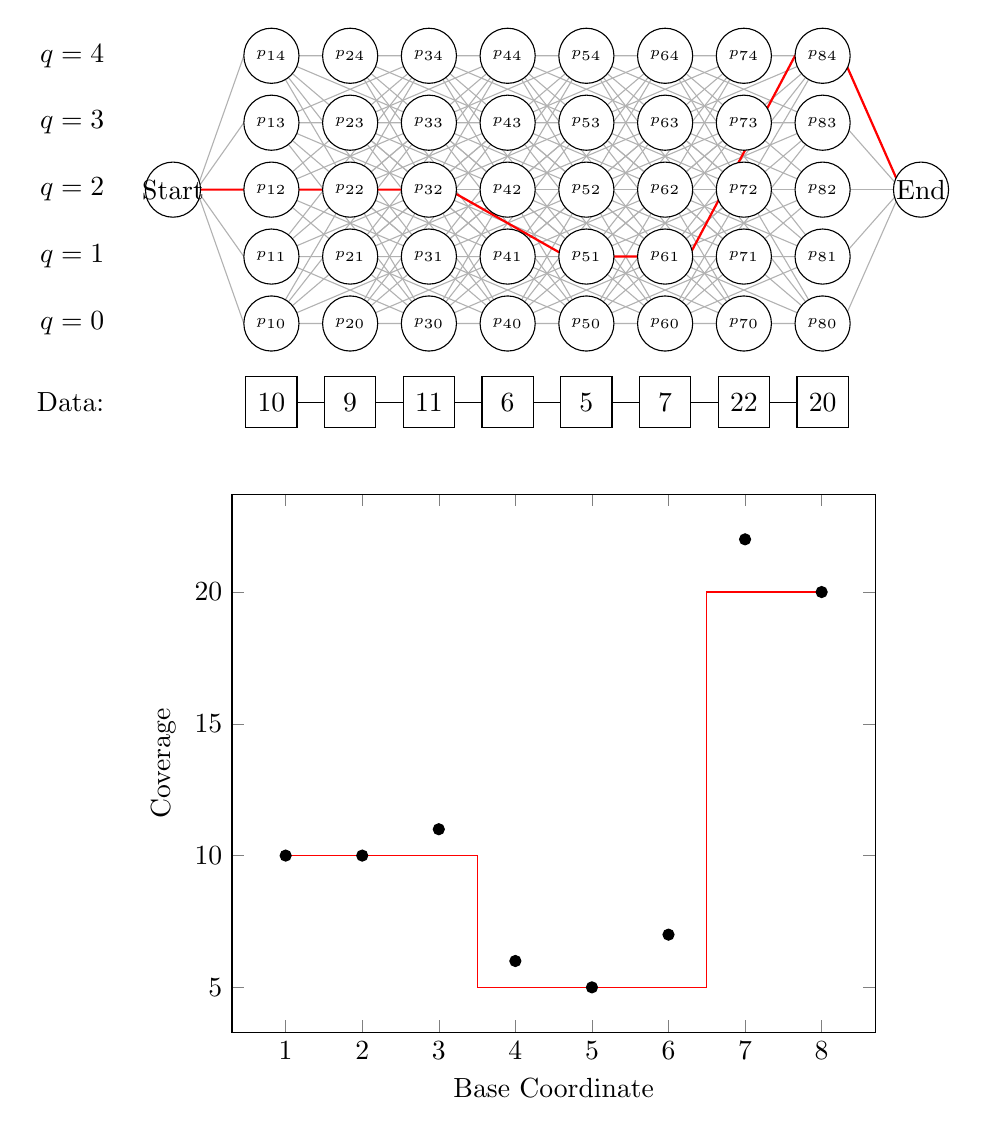
\begin{tikzpicture}
							
						%%network 
							\node[anchor=east] at (-2,0) {Data:};
							\draw (0,0)--++(7,0);
							\def\w{0.65}
							\foreach[count=\i] \j in {10,9,11,6,5,7,22,20}
							{
								% \draw[fill=white] (\i-1,0) circle (0.35);
								\draw[fill=white] ({\i-1-\w/2},{\w/2})--({\i-1+\w/2},{\w/2})--({\i-1+\w/2},{-\w/2})--({\i-1-\w/2},{-\w/2})--cycle;
								\node at (\i-1,0) {$\j$};
							}
							
							
							
							\def\fac{0.85}
							\foreach \q in {0,...,4}
							{
								\def\y{\fac*\q+1}
								\draw[black!30!white] (-0.95,{2*\fac+1})--(-0.35,\y)--(7.25,\y)--(8,{2*\fac+1});

								\foreach \i in {0,...,5}
								{
									\foreach \qq in {0,...,4}
									{
										\if\q\qq

										\else
											\draw[black!30!white] (\i,{\q*\fac+1})--(\i+2,{\qq*\fac+1});
										\fi
									}
								}
							}

							\draw[red,thick] (-0.95,{2*\fac+1})--(2.25,{2*\fac+1})--(3.75,{\fac+1})--(5,{\fac+1})--++(0.3,0)--(6.65,{4*\fac+1})--(7.25,{4*\fac+1})--(8,{2*\fac+1});
							
							\foreach \q in {0,...,4}
							{
								\def\y{\fac*\q+1}
								% \draw (4.25,\y)--(6,\y);
								\node[anchor=east] at (-2,\y) {$q=\q$};
								\foreach \i in {1,...,8}
								{
									
									\draw[fill=white] (\i-1,\y) circle (0.35);
									% \draw[fill=white] ({\i-1-\w/2},{\w/2})--({\i-1+\w/2},{\w/2})--({\i-1+\w/2},{-\w/2})--({\i-1-\w/2},{-\w/2})--cycle;
									\node at (\i-1,\y) {\tiny $p_{\i\q}$};
				
								}
								
								
							}
							\draw[fill=white] (-1.25,{2*\fac+1}) circle (0.35);
							\node at (-1.25,{2*\fac+1}) {Start};
							\draw[fill=white] (8.25,{2*\fac+1}) circle (0.35);
							\node at (8.25,{2*\fac+1}) {End};

						%%plot
							\begin{axis}[width=9.75cm,xlabel={Base Coordinate},ylabel={Coverage},at={(-0.5cm,-8cm)},scatter/classes={%
								a={mark=o,fill=black}}]
								\addplot[only marks,scatter src=explicit symbolic] table[row sep=crcr]{
									x y label \\
									1 10 a\\
									2 10 a\\
									3 11 a\\
									4 6 a\\
									5 5 a\\
									6 7 a\\
									7 22 a\\
									8 20 a\\
								};

								\addplot[red] table[row sep=crcr]{
									x y label \\
									1 10 a\\
									2 10 a\\
									3 10 a\\
									3.5 10 a\\
									3.5 5 a\\
									5 5 a\\
									6 5 a\\
									6.5 5 a\\
									6.5 20 a\\
									8 20 a\\
								};
								
								
							\end{axis}
						\end{tikzpicture}
						}
						\caption{(Top panel) A demonstration of an optimal path through a network with $L=2$ and $\nu=5$, given some example coverage data. (Bottom panel) a projection of this path back onto the coverage distribution. For aesthetic reasons we have placed the transitions at half-integers -- in practice non-integer values of base index are meaningless.}\label{F:Path}
					\end{center}
				\end{figure}
		% \section{Harmonic Tree}

		% 	The Harmonic approach shows a vast improvement over the other methods -- however it still has a number of issues -- primarily revolving around the `smoothing' aspect. Simply put: the most obvious (continuous) ways of enforcing smoothness tends to be to `bind' subsequent points together with a 'cost function' associated with moving away from the surrounding points. 

		% 	This works, but has the problem of `fine tuning': the prior has a `strength' as an external parameter, which then controls the `spikiness' of the output curve. By selecting this value appropriately, the user is able to either make the output ust as much of a forest as the input data, or perfectly smooth: and anything in between. 

		% 	The user is then left to fine tune the dials of this parameter until they get something they would find acceptable. The problem with this is that it invariably leaves the user projecting their own expectations on the input -- you only get out what you put in. 

		% 	In such a case, a Bayesian statistician would say that we have formulated our Prior poorly -- it has a free parameter (the strength), over which we have actually no prior knowledge. In fact, on further examination the strength (which is usually formulated as a length scale over which the binding happens) isn't even the quantity we are wishing to constrain since!
			
		% 	% We might therefore wish to come up with a more mechanistic way of imposing these constraints. We will still have a free parameter(s) (any kind of prior will require this), but we might be able to express them in ways which make the numbers harder to `fudge'. 
			
		% 	We must therefore ask what it is we wish our smoothing-prior to do since it evidently isn't `smoothing' -- since we are looking for a highly discontinuous output function! We want our prior to be such that it causes the model to disregard small-scale oscillations in the coverage as merely being noise. Smoothing length scales had this as a side effect -- but with the unfortunate side effect that they also smoothed over what we (probably) believe to be sharp, discontinuous edges. 

		% 	Let us therefore use this as a strict prior: there should be no oscillations on a scale shorter than some enforced length scale $L$ - we assert that any gains or losses which span $L$ bases or fewer are merely noise. Any determination if a change in harmonic has occurred must therefore consider \textit{at least} $L$ bases. 

		% 	A standard Bayesian hypothesis can be formulated at the index $i$ to determine if there has been a transition by considering the Hypothesis ``the harmonic on the domain $[q,q+L]$ is equal to $q_i$'', and testing all reasonable values of $q_i$ (we suggest between 0 and 10 as being reasonable values). The odds-Likelihood of a transition is then:
		% 	\begin{equation}
		% 		p(\text{transition } q_{i-1} \to q) = \frac{p(D_i\to D_{i+L| q})}{p(D_i\to D_{i+L| q_{i-1}})} \times \text{Prior}(q | q_{i-1})
		% 	\end{equation}
		% 	It simply suffices to find if any of these terms is greater than 1 and, if any, which is the largest: this is the assigned value of $q$. The prior then allows us to penalise `marginal' jumps by only assigned jumps when the evidence reaches a threshold:
		% 	\begin{equation}
		% 		\text{Prior}(q | q_{i-1}) = \begin{cases} 0 < \alpha \leq 1 & \text{ if } q = q_{i-1}
		% 		\\
		% 	1 & \text{else}\end{cases}
		% 	\end{equation}
		% 	The case where $\alpha \approx 1$ means we accept a transition when the evidence is very marginal, $\alpha \ll 1$ means we require an overwhelming amount of evidence. Given some of the other post-processing that we will be doing (to locate transition edges more precisely), and provided $L$ is sufficiently large that most spurious jumps will be eliminated, we use $\alpha = 0.5$ as a good first port of call.

		% 	Should we find that $q \neq q_{i-1}$, we have therefore been able to robustly identify that there is a transition in the region $[i,i+L]$ - but it is not true that the transition edge is at $i$ -- if $\alpha = 1$ the transition is probably somewhere in the middle of the region, whilst as $\alpha \to 0$ it gets closer to $i$. To robustly identify the edge of the transition we need to do a second hypothesis test -- that the transition $q_{i-1} \to q$ occurs at an index $j$, the Likelihood of which is computed as:
		% 	\begin{equation}
		% 		\mathfrak{p}(\text{transition at} j | i, \text{data, }D) = p(D_i \to D_{j-1} | q_{-1} ) \times p(D_j \to D_{j + L} | q)
		% 	\end{equation}
		% 	I.e., we sucessively compute the probability that every point left of $j$ is at the original $q=q_{i-1}$, and every point to the right is at the new value of $q$: the one with the highest value of $\mathfrak{p}$ is where we assign $j$.

		% 	Having now determined the value of $j$ and $q_j$, we jump to index $j+L$ and continue the search looking for the next transition, repeating this process until each transition has been identified. The only parameters in this model are the minimum size of a transition `block', $L$, and $\alpha$, the amount of evidence needed before we accept that a transition is present in a region. 

		% 	All that remains is to compute the quantity $p(D_i \to D_j)$ - we can do this using either the simple Poisson structure, or the error-accounting methods of the previous section. Since we are assuming that the probabilities are independent (the non-independence being enforced by the structure of our algorithm), it then is a simple matter of computing the product of these terms. In practice, however, it is probably more convenient to compute these in logarithmic space.

		% 	Hence:
		% 	\begin{align}
		% 		\mathcal{P}(i|q,q_{i-1}) & = \sum_{n = 0}^{L-1} \log\left( p(D_{i+n} | q) \right) + \log\left(\text{Prior}(q | q_{i-1})\right)
		% 		\\
		% 		p(D_j | q)  & = \sum_{k} {NB}\left(k; \frac{q^2\nu^2}{\sigma^2}, \frac{q\nu}{q\nu + \sigma^2} \right) \times p(D_j|k)
		% 		\\
		% 		p(D_j|k) &= \mathcal{N} \exp(-(D_j-k)^2/(2 \gamma^2))
		% 	\end{align}
		% 	This model has five parameters: $L$, the minimum transition size, $\alpha$, the evidence weighting, $\nu$ the global fundamental frequency, $\sigma$, the dispersion of the underlying mechanism and $\gamma$, the standard error in the assigned coverage values. Of these, three must be assigned \textit{a priori} by the user: $\alpha$, $L$ and $\gamma$.

		% 	This computation can be streamlined in many ways: the NB function can be pre-tabulated for every $0 \leq k < k_\text{max}$ $0 \leq q < q_\text{max}$ every time a new $\nu$ and $\sigma$ are formulated since, by definition, they will all be called at least once -- and some values of $k$ will be called many thousands of times. 
		% 	% We can then assume that all values of $q$ between $i$ and $i+L$ are equal to this value of $q$ - and so we make a jump to $

		% 	\begin{figure}
		% 		% \includegraphics*[width=\linewidth,keepaspectratio=true]{Figure_1.png}
		% 		\caption{A demonstration of how the different probability models assign slightly different values of the resonance $q$ given otherwise identical parameters -- as expected, this mostly occurs at the borders of where a transition occurs. The only truly notable difference is the `Error Prone Method', in which we sum over nearby $k^\prime$, in that this permits non-zero values of $k$ to be considered for the zeroth order resonance -- the other methods preclude considering any $k>0$ (or any gap containing $k>0$) as the zeroth resonance, which can lead the model to assume that deleted regions have not been deleted.}
		% 	\end{figure}

	% \subsubsection{An Alternative Formulation}

	% 		We have formulated this approach in terms of a series of Bayesian Inferences -- though this is far from the only way to think about what we are doing here. 

	% 		An equally valid approach would be to consider this as a curve fitting exercise, where the functional form we are attempting to fit is:

	% 		\begin{spalign}
	% 			f(x| \{q_i, \nu, t_i \}) & = \nu \left(q_0 + \sum_i^N (q_i - q_{i-1}) \theta(x - t_i)) \right)
	% 			\\
	% 			q_i \in \mathbb{Z}_0
	% 			\\
	% 			\nu, t_i \in \mathbb{R}
	% 		\end{spalign}
	% 		That is, the function can be thought of a series of Heaviside Step functions ($\theta(x)$) - the Harmonic restriction can clearly be seen once again in the restriction that $q \in \mathbb{Z}_0$, i.e. it must be an integer (or zero).

	% 		The mechanism for finding the most likely value of the curve parameters is identical to those we have previously discussed, however by fixing $N$ as some large number this provides a fixed-length encoding, ideal for input into a neural network.
\end{document}
